\documentclass{book}
\usepackage{booktabs}
\usepackage{geometry}
\usepackage{enumerate}
\usepackage{setspace}
\usepackage{amsthm}
\usepackage{float}
\usepackage{color, soul}
\usepackage{amsmath,amssymb}
\usepackage{amstext}
\usepackage{makecell}
\usepackage{subfigure}
\usepackage{graphicx}
\usepackage{array}
\begin{document}
{\huge 4.1 Projectile motion with air drag}

{\Large 1.}
\vspace{0.01\textheight}
According to the formular for acceleration:
{\"r}$=-g-\frac{k}{m}v$

$\begin{cases}
    v_{x_{0}}= & v_{0}cos\alpha \\

    v_{y_{0}}= & v_{0}sin\alpha
  \end{cases}$
\quad $
  \begin{cases}
    a_{x_{i}}= & -\frac{k}{m}v_{x_{i}}   \\

    a_{y_{i}}= & -g-\frac{k}{m}v_{y_{i}}
  \end{cases}
$

\vspace{0.01\textheight}
Using Euler's method:
\vspace{0.01\textheight}

\quad $
  \begin{cases}
    v_{x_{i+1}}= & v_{x_{i}}+a_{x_{i}}\Delta t = v_{x_{i}}(1-\frac{k}{m}\Delta t)           \\

    v_{y_{i+1}}= & v_{y_{i}}+a_{y_{i}}\Delta t = v_{y_{i}}(1-\frac{k}{m}\Delta t)-g\Delta t
  \end{cases}
$

\vspace{0.01\textheight}

\quad $
  \begin{cases}
    x_{i+1}= & x_{i}+v_{x_{i}}\Delta t \\

    y_{i+1}= & y_{i}+v_{y_{i}}\Delta t
  \end{cases}
$

\vspace{0.01\textheight}
{\Large 2.}
The initial conditions are set as: $x_{0}=y_{0}=0, \alpha =\frac{\pi}{6}$.

The following graph in Figure 1 shows that the numerical result is not sensitive to the choice of the step {$\Delta t$}

\begin{figure}[H]
  \centering
  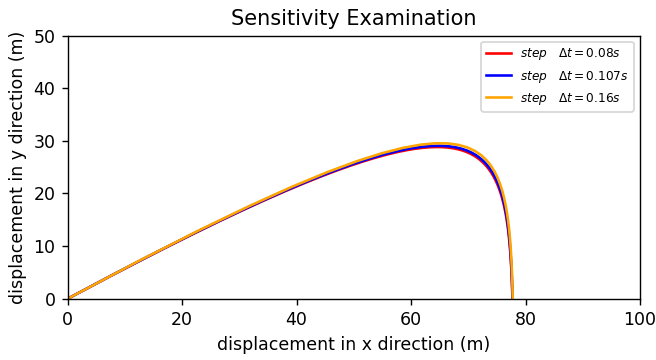
\includegraphics[width=11cm,height=6cm]{./graphs/project4.1.2(4).png}
  \caption{4.1.2(1). Examine the sensitivity of the numerical result to the choice of the step $\Delta t$}
\end{figure}

\quad The analytical result is given as:

\quad $\begin{cases}
    x(t)= & v_{0}cos\alpha \cdot \frac{m}{k}(1-e^{-\frac{k}{m}t})                          \\
    y(t)= & (v_{0}sin\alpha + \frac{mg}{k})\frac{m}{k}(1-e^{-\frac{k}{m}t})-\frac{mg}{k}t)
  \end{cases}$

With the analytical formulas and numerical values, three trajectories for different steps of time are plotted in as belows:

The red lines are the trajectories plotted using Euler's method, and the blue lines are trajectories plotted using analytical formulas. It can be observed from the graphs in Figure 2 that, the analytical formulas and numerical formulas reach quite close results, and smaller steps of time can lead to better approximation to the result.
\begin{figure}[H]
  \centering
  \subfigure[$\Delta t=0.08s$]{
    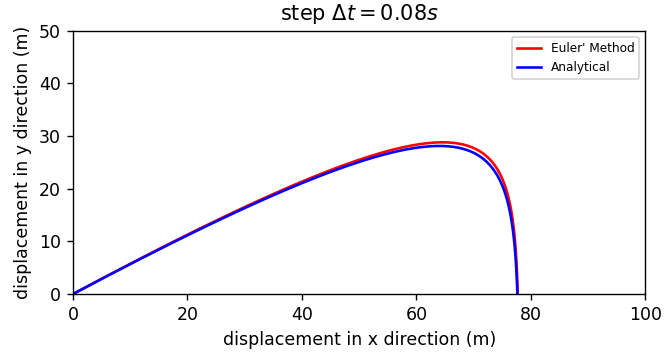
\includegraphics[scale=0.32]{./graphs/project4.1.2(1).png}}
  \hspace{0.05in}
  \subfigure[$\Delta t=0.107s$]{
    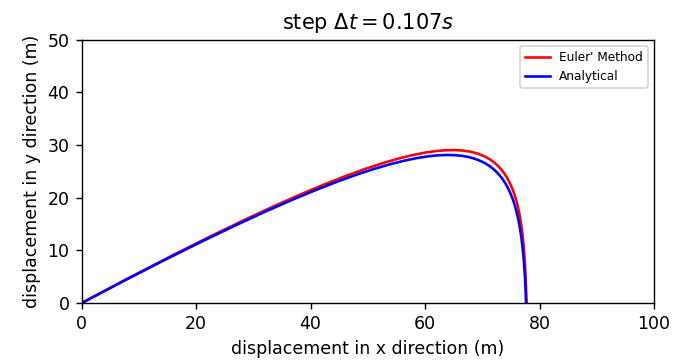
\includegraphics[scale=0.32]{./graphs/project4.1.2(2).png}}
  \hspace{0.05in}
  \subfigure[$\Delta t=0.16s$]{
    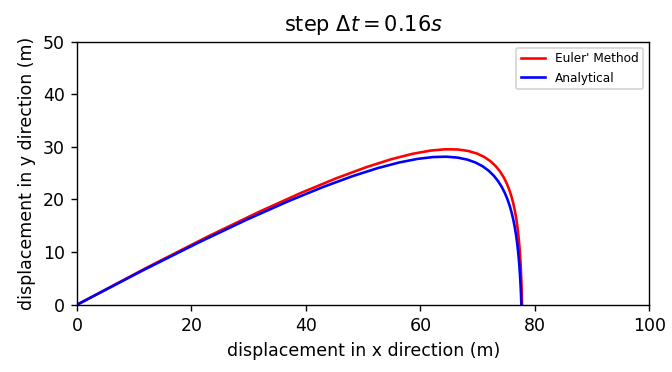
\includegraphics[scale=0.32]{./graphs/project4.1.2(3).png}}
  \caption{4.1.2(2). Plot the trajectories for three different values of $\Delta t$}
\end{figure}

{\Large 3.(a)}
\begin{figure}[H]
  \centering
  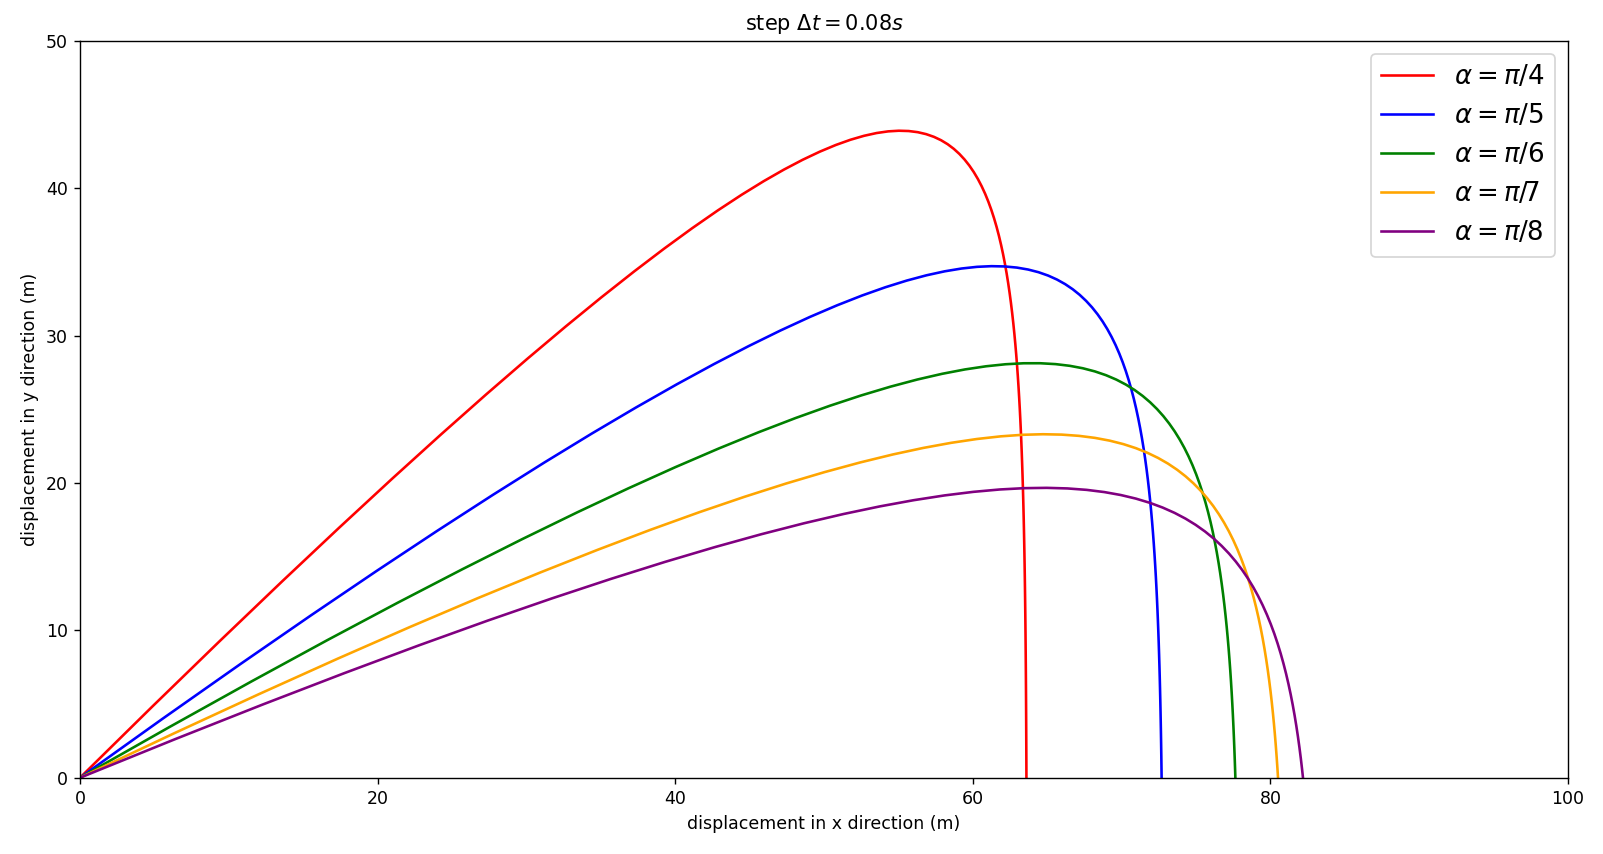
\includegraphics[scale=0.4]{./graphs/project4.1.3(a).png}
  \caption{4.1.3(a). Plot five trajectories for different initial angles}
\end{figure}
Choose the step to be 0.08s.
The initial speed of the projectile is fixed to be 90m/s, and the problem is solved numerically for five different values of angles.
  {The five angles are selected to be $\frac{\pi}{4},\frac{\pi}{5},\frac{\pi}{6},\frac{\pi}{7},\frac{\pi}{8}.$}, and the graph is shown in Figure 3.

The shape of the trajectories are quite similar as all of them increasely steadily and then precipitate sharply.
It can be observed the figure that, the larger the initial angle to the horizontal is, the higher the maximum height is, and the shorter the range is.

\newpage
{\Large 3.(b)}
\begin{figure}[H]
  \centering
  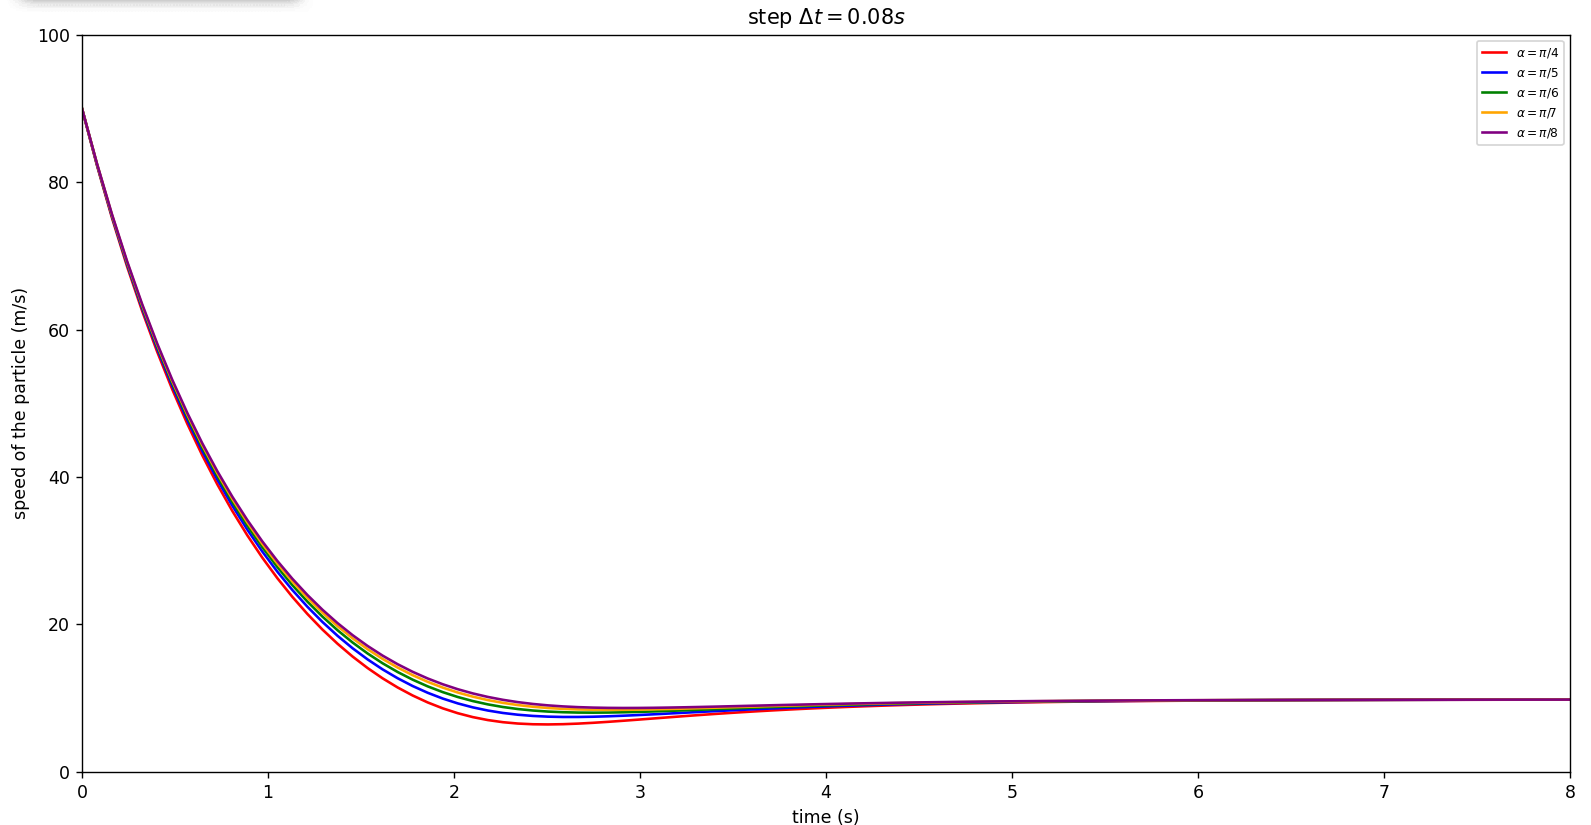
\includegraphics[scale=0.4]{./graphs/project4.1.3(b).png}
  \caption{4.1.3(b). Plot the time dependence of the speed of the particle for different initial angles}
\end{figure}
It can be observed from the graph in Figure 4 that, the speed of the particle drops quickly at the first several seconds, and then the speed become stable.

\vspace{0.03\textheight}
{\Large 4.(a)}
\begin{figure}[H]
  \centering
  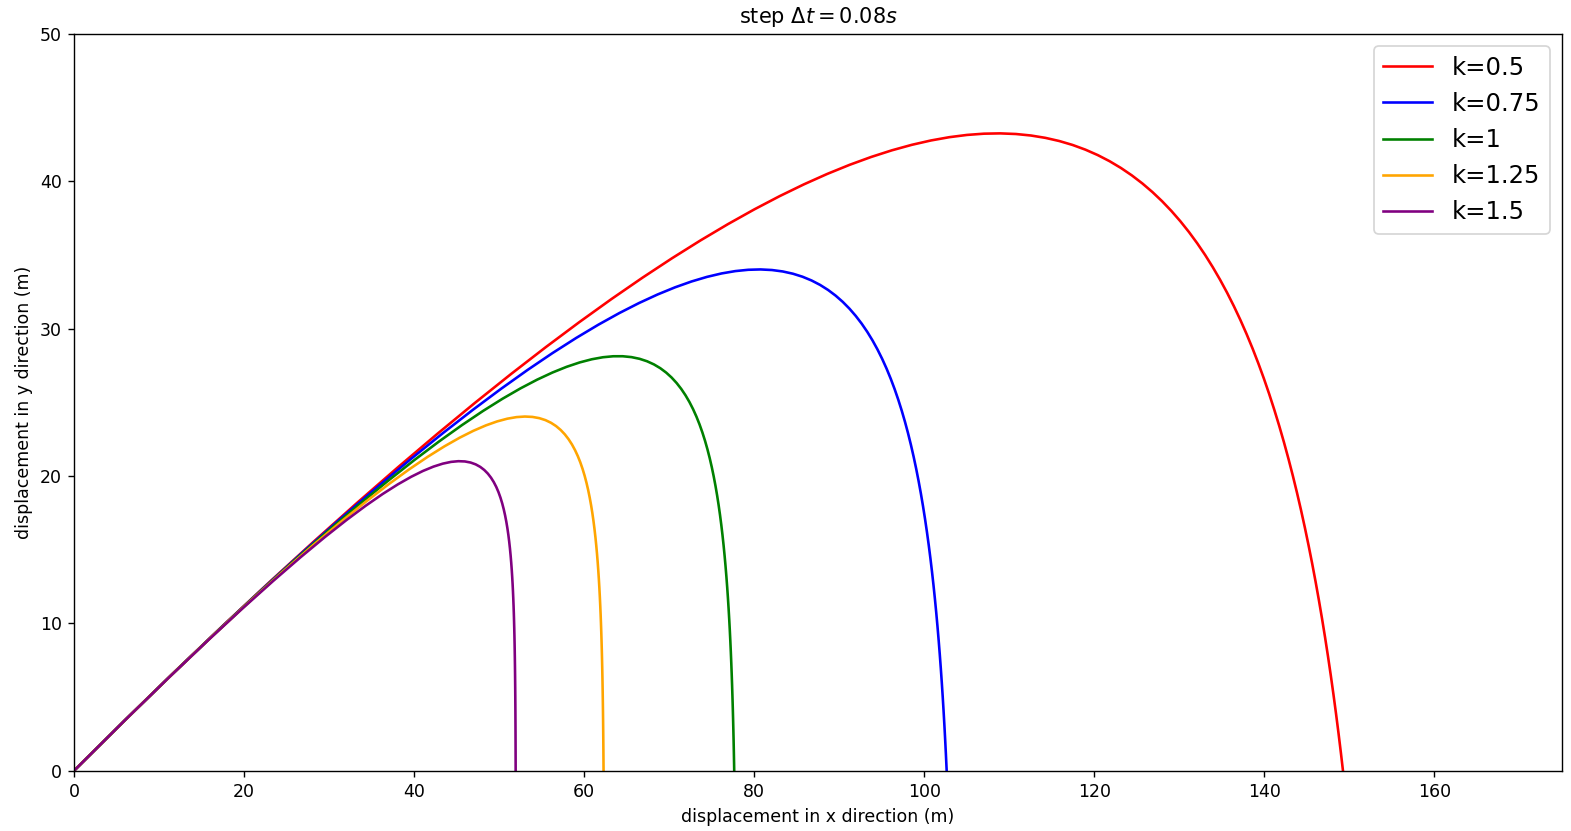
\includegraphics[scale=0.4]{./graphs/project4.1.4(a).png}
  \caption{4.1.4(a). Plot five trajectories for different drag coefficient k}
\end{figure}
\vspace{0.01\textheight}
The initial speed of the projectile is fixed to be 90m/s, and the initial angle is set to be $\pi/6$. Five different values for k is selected as 0.5,0.75,1,1.25 and 1.5.

From the graph in Figure 5, it can be observed that the larger the drag coefficient k is, the lower the maximum height is, and the shorter the range of the projectile is.

  {\Large 4.(b)}

\begin{figure}[H]
  \centering
  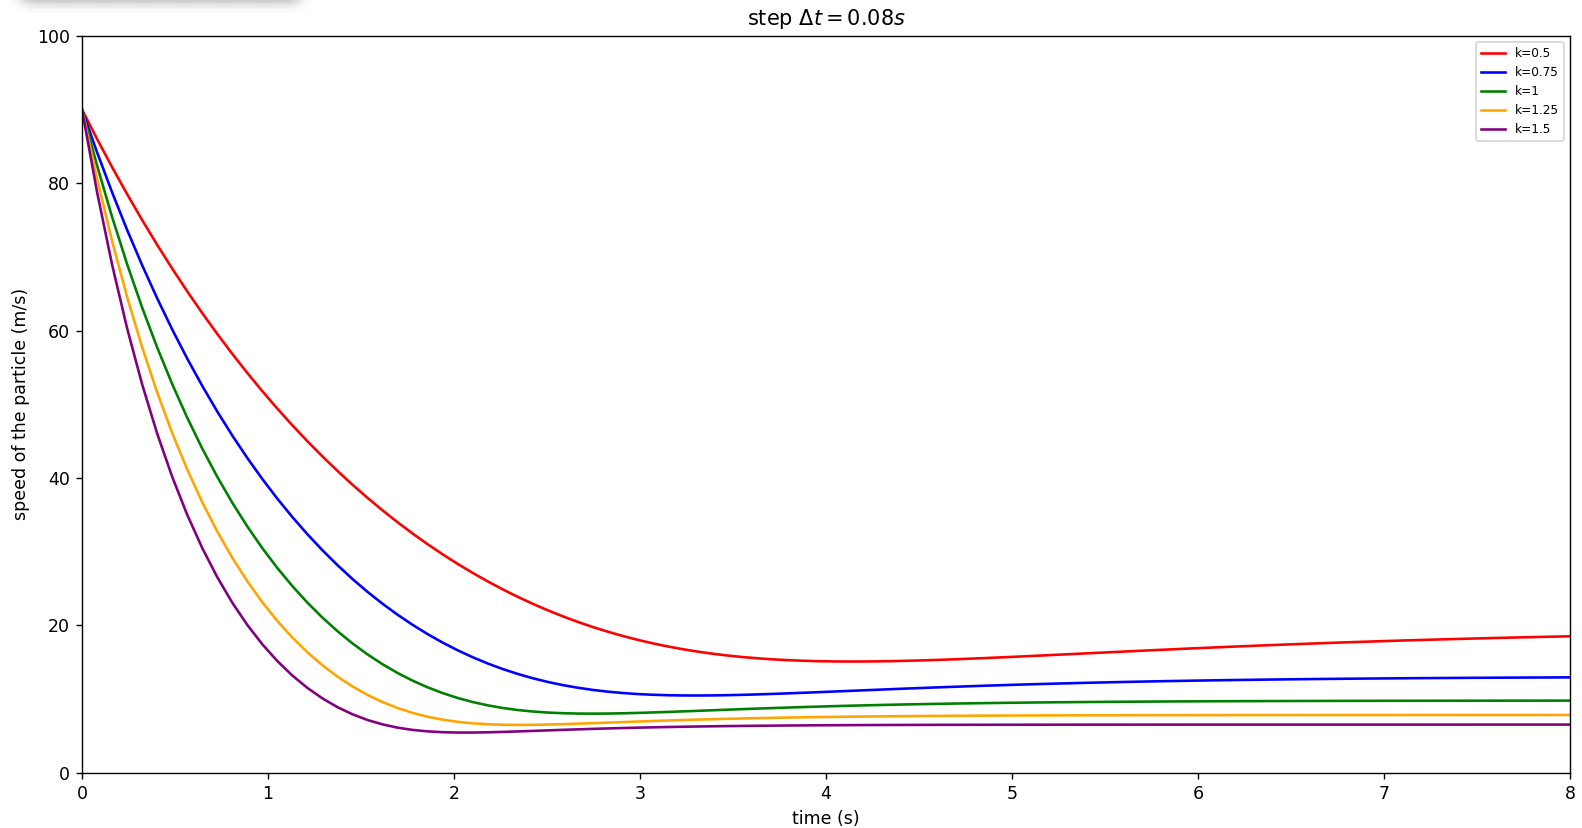
\includegraphics[scale=0.4]{./graphs/project4.1.4(b).png}
  \caption{4.1.4(b). Plot the time dependence of the speed of the particle for different drag coefficient k}
\end{figure}

It can be observed from the graph in Figure 6 that, the speed of the particle drops quickly at the first several seconds, and then the speed become stable.
A tendency can also be clearly noticed that the larger the drag coefficient k is, the smaller the speed of the particle is at any instance of time.

\vspace{0.01\textheight}
{\Large 5.} According to the formula for acceleration: {\"r}=$-g-\beta |v|v=-g-\frac{b}{m}|v|v$

$\begin{cases}
    v_{x_{0}}= & v_{0}cos\alpha \\

    v_{y_{0}}= & v_{0}sin\alpha
  \end{cases}$
\quad $
  \begin{cases}
    a_{x_{i}}= & -\frac{b}{m} \sqrt{v_{x_{i}}^{2}+v_{y_{i}}^{2}}v_{x_{i}}   \\

    a_{y_{i}}= & -g-\frac{b}{m} \sqrt{v_{x_{i}}^{2}+v_{y_{i}}^{2}}v_{y_{i}}
  \end{cases}
$

\vspace{0.01\textheight}
Using Euler's method:
\vspace{0.01\textheight}

$\begin{cases}
    v_{x_{i+1}}= & v_{x_{i}}(1-\frac{b}{m}\sqrt{v_{x_{i}}^{2}+v_{y_{i}}^{2}}\Delta t)            \\

    v_{y_{i+1}}= & -g\Delta t+v_{y_{i}}(1-\frac{b}{m}\sqrt{v_{x_{i}}^{2}+v_{y_{i}}^{2}}\Delta t)
  \end{cases}$

\vspace{0.006\textheight}
$
  \begin{cases}
    x_{i+1}= & x_{i}+v_{x_{i}}\Delta t \\

    y_{i+1}= & y_{i}+v_{y_{i}}\Delta t
  \end{cases}
$

\newpage
{\Large 6.}
\begin{figure}[H]
  \centering
  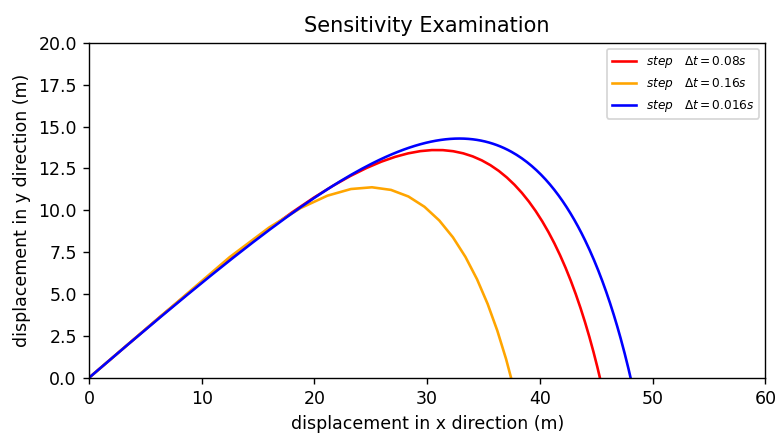
\includegraphics[scale=0.6]{./graphs/project4.1.6.png}
  \caption{4.1.6. Examine the sensitivity of the numerical result to the choice of the step $\Delta t$}
\end{figure}
Three trajectories are plotted according to three different values of {$\Delta t$}, which are respectively 0.16s 0.08s,and 0.016s.
It can be ovserved from the graph in Figure 7 that, the numerical result is sensitive to the choice of the step {$\Delta t$}.

\vspace{0.01\textheight}
{\Large 7(a).}
\begin{figure}[H]
  \centering
  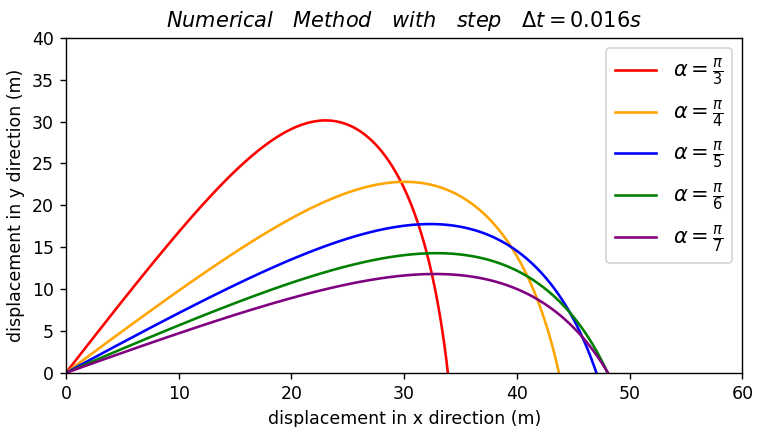
\includegraphics[scale=0.6]{./graphs/project4.1.7(a).png}
  \caption{4.1.7(a). Plot five trajectories for different initial angles}
\end{figure}
The initial speed is fixed to be 90m/s, and the drag coefficient is fixed to be 0.05.

Five trajectories are plotted for different initial angles to the horizontal, which are respectively {$\pi/3,\pi/4,\pi/5,\pi/6,\pi/7$}

It can be observed from the graph in Figure 8 that, the shape of the trajectories follows the pattern that the curve first gradually rises and then declines quickly.
A trend can also be noticed that the larger the initial angle is, the higher the maximum height is, and the shorter the range is.

\vspace{0.01\textheight}
{\Large 7(b).}
\begin{figure}[H]
  \centering
  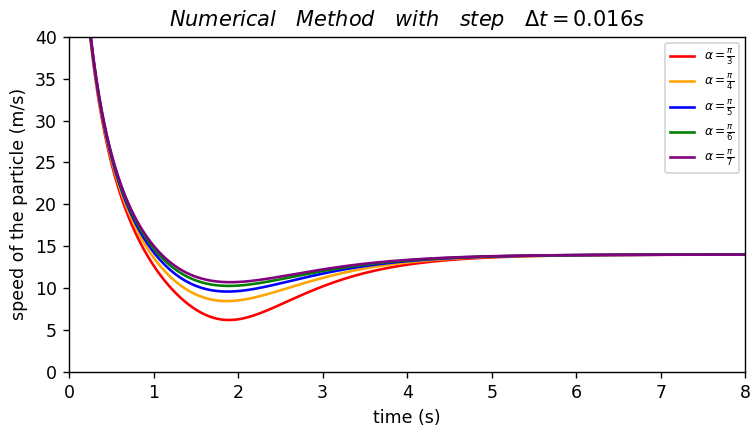
\includegraphics[width=9cm,height=6cm]{./graphs/project4.1.7(b).png}
  \caption{4.1.7(b). Plot the time dependence of the speed of the particle for different initial angles}
\end{figure}
The initial speed is fixed to be 90m/s, and the drag coefficient is fixed to be 0.05.
Different initial angles are selected to be {$\pi/3,\pi/4,\pi/5,\pi/6,\pi/7$}.
It can be observed from the graph in Figure 9 that, the speed follows a certain pattern for different inital angles that the speed first declines quickly, and then rises a bit, and finally becomes stable.
A trend can be noticed that, the larger the inital angle, the quicker the speed declines at the beginning, and the speed turns out be slower at any instance of time.

\vspace{0.01\textheight}
{\Large 8(a).}
\begin{figure}[H]
  \centering
  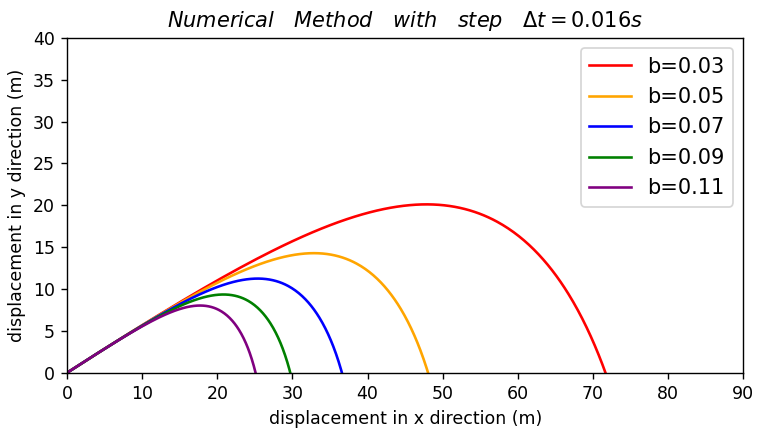
\includegraphics[scale=0.6]{./graphs/project4.1.8(a).png}
  \caption{4.1.8(a). Plot five trajectories for different drag coefficients b}
\end{figure}
The initial speed is fixed to be 90m/s, and the inital angle of speed to the horizontal is fixed to be {$\pi/6$}.
Five trajectories are plotted using the numerical method with respect to 5 different drag coefficients b, which are 0.03,0.05,0.07,0.09 and 0.11.

It can be observed from the graph in Figure 10 that, the shape of the trajectories is that the curve first rise gradually and then decline quickly.
It can be also be noticed that the large the drag coefficient b is, the lower the maximum height is, and the shorter the range is.

\vspace{0.01\textheight}
{\Large 8(b).}
\begin{figure}[H]
  \centering
  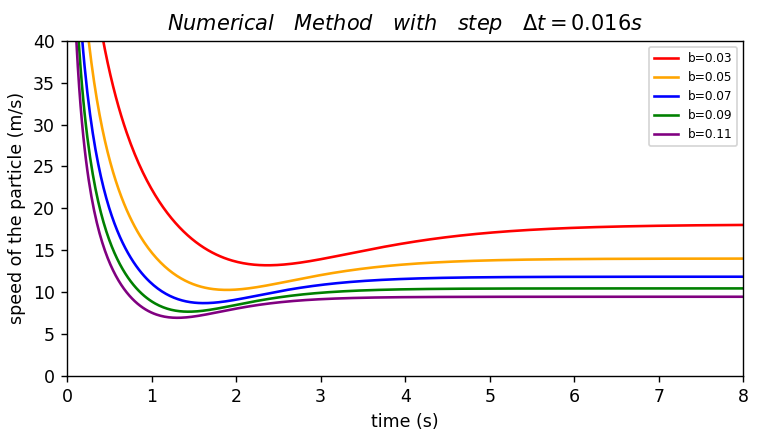
\includegraphics[scale=0.4]{./graphs/project4.1.8(b).png}
  \caption{4.1.8(b). Plot the time dependence of the speed of the particle for different drag coefficients}
\end{figure}
The initial speed is fixed to be 90m/s, and the inital angle of speed to the horizontal is fixed to be {$\pi/6$}.
Different drag coefficients are selected to be 0.03,0.05,0.07,0.09 and 0.11.

It can be observed from the graph in Figure 11 that, the speed follows a certain pattern for different drag coefficients that the speed first declines quickly, and then rises a bit, and finally becomes stable.

A trend can be noticed that the larger the drag coefficient is, the quicker the speed declines at the beginning, and the speed is slower at any instance of time.

\vspace{0.02\textheight}
{\Large 9.}
\begin{figure}[H]
  \centering
  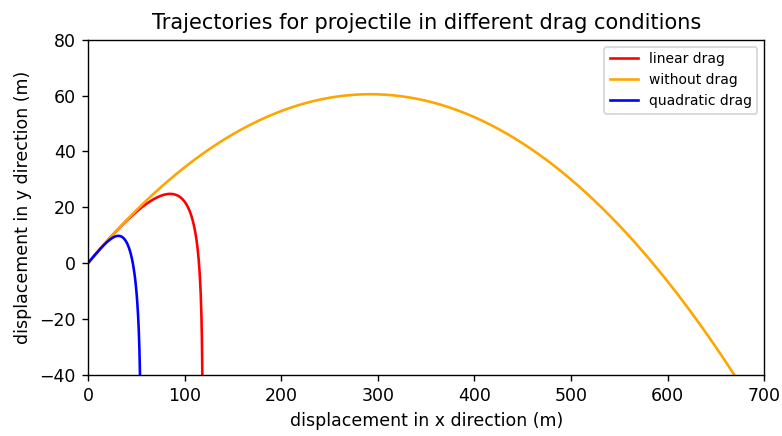
\includegraphics[scale=0.4]{./graphs/project4.1.9.png}
  \caption{4.1.9. Plot the trajectories for projectiles in different drag conditions}
\end{figure}
The initial speed is 90m/s, and the initial angle to the horizontal is {$\frac{\pi}{8}$}.
To choose the drag coefficients to let the terminal speeds equal, by calculating the terminal speed:

\quad$
  \begin{cases}
    v_{terminal_{linear}}= & \frac{mg}{k}        \\

    v_{terminal_{quad}}=   & \sqrt{\frac{mg}{b}}
  \end{cases}
$
\quad ,\quad So $\frac{mg}{k}=\sqrt{\frac{mg}{b}}$

$k=\sqrt{gb}$. Let b=0.05 and k=0.7, so that the terminal speeds for linear drag condition and quadratic drag condition are the same.

Plug in the drag coefficients, and the final graph is plotted in Figure 12.
\end{document}